\section{Experiment Methodology}
\label{sec:experiment}

In the experiment, we only consider single precision, real number matrix multiplication. 
\par
We implement an exhaustive search on ATLAS and the space of each parameter are chosen as follows.\par
$NB$: Multiple of 4 in range $[20, 80]$\par
$MU$,$NU$: $\{1, 2, 3, 4, 5, 6, 8, 10, 12\}$ for 16 registers,
		\{4, 6, 8, 10, 12, 14, 16, 24, 32\} for 32 registers\par
$KU$: $\{1, 2, 3, 4, 5, 6, 8, 10, 12, NB\}$\par
The exhaustive search tries every possible combination of them. 
On a typical platform as we mentioned in Section \ref{sec:atlas_intro}, it takes more than 10 hours to finish 
the search on 12960 data points.\par

We evaluate the result on 12 platform, as shown in Figure \ref{fig:platforms}. \textit{arma7} and \textit{arma15}
are two ARM Cortex processors on an ODROID board. 
\textit{ypei\_mac} and \textit{michael\_mac} are two perfernal MAC laptops 
with Intel CORE i7 processors. The rest eight platforms are machines of ICES or CS department. They are all intel processors.\par

Note that the third column \textit{architecture} is a category provided by ATLAS configuration. 
ATLAS identifies this information but does not use it in the orthogonal search procedure. Instead, after automatically 
generating high performance code, ATLAS compares it with existing hand-tuned unleashed codes which has been included in the system, 
and pick the best. Those hand-written codes are categorized according to this \textit{architecture}. 
We adopt it as one of our training set grouping metric in the experiment.\par



\begin{figure*}[tbhp]
  \centering
  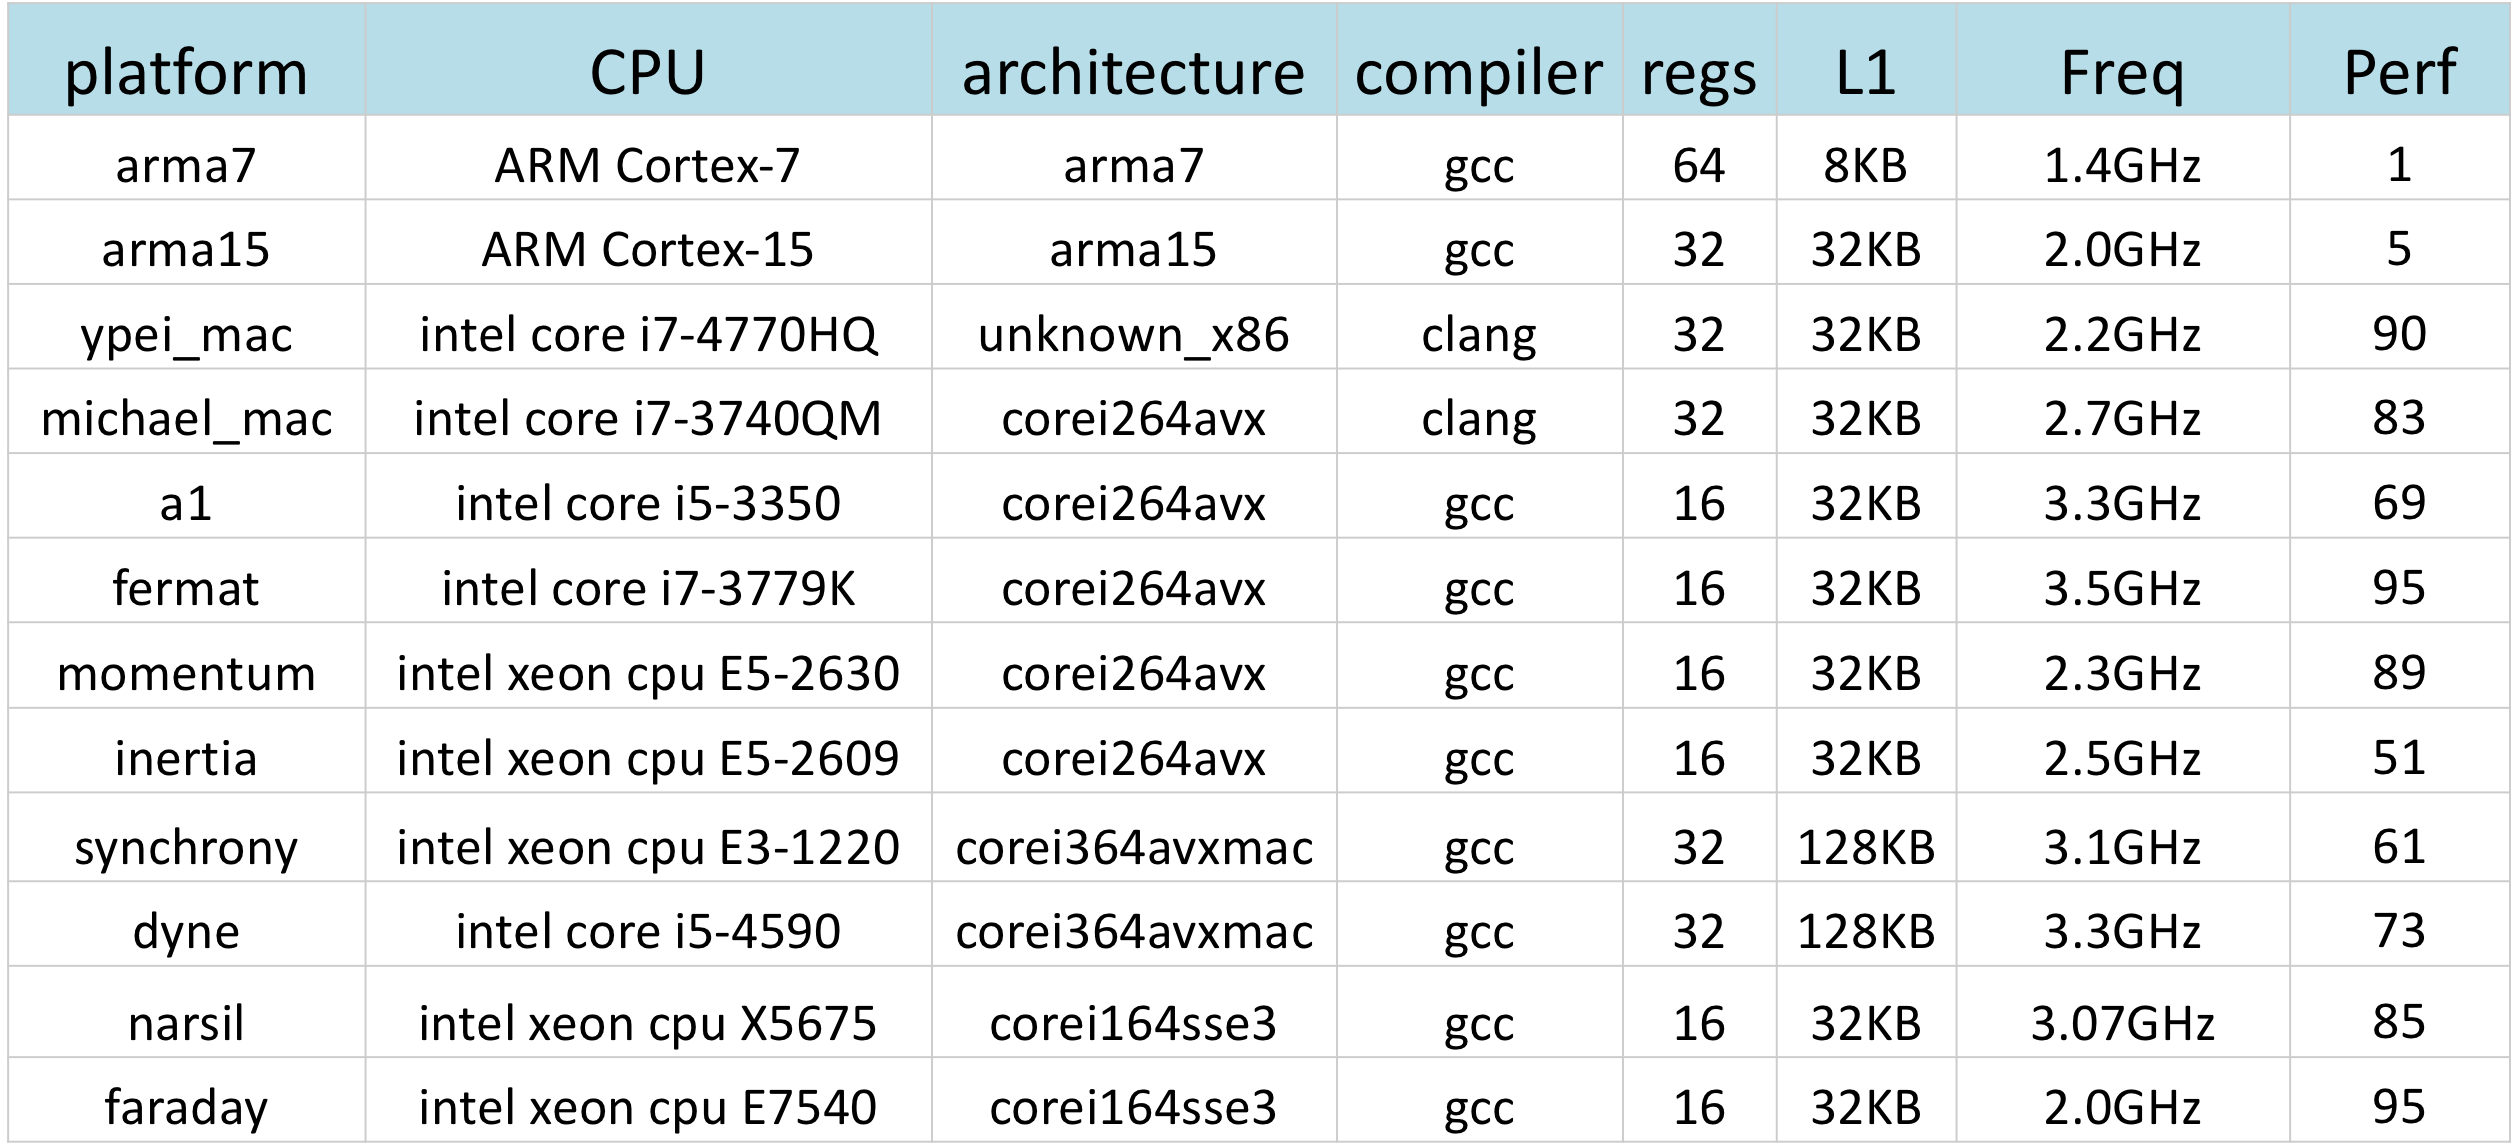
\includegraphics[width=0.9\textwidth]{images/platforms.png}
  \caption{Platforms profiled in this paper}
  \label{fig:platforms}
\end{figure*}


In the experiment, we train the model offline from a training set of platforms, and get the top ten knob settings generated from the model.
We evaluate these ten knob settings on another target platform and compare it with the best of exhaustive search. We select 
three catogories of training sets. 1) ALL except the target. 2) "Corei" architecture group. This group is all the platforms 
with intel precessors except \textit{ypei\_mac} since ATLAS is unable to identify its architecture. 3) Specific architecture group.
We categorize the platform spcifically according to the architure. Each artchiture conresponds to a group and we only use data 
from the exact same architure to train. \par

We picked 3 different models M5, bagging predictor and extremely randomized tree from capri. We evaluate each training model on each training 
set individually.


